\section{Chlorophyllkataboliten des Brokkoliblattes mithilfe von LC-MS identifiziert}

\subsection{Auswertung der Chromatogramme}

Mithilfe einer \gls{hplc} kann bestimmt werden, ob es sich bei einem bestimmten \gls{Chl-K} um einen NCC, DNCC, YCC oder DYCC handelt. Das Chromatogramm in Abbildung \ref{fig:HPLCChromatogramm} zeigt, welche der Kataboliten mithilfe ihrer UV/Vis Spektren identifiziert werden konnten. Es dürfte sich dabei ob ihrer etwas höheren Intensitäten um die Hauptkataboliten des Brokkoliblattes handeln. Dies müsste jedoch über gezielte quantitative Messungen weiter und genauer untersucht werden.

\begin{figure}[!htbp]
  
  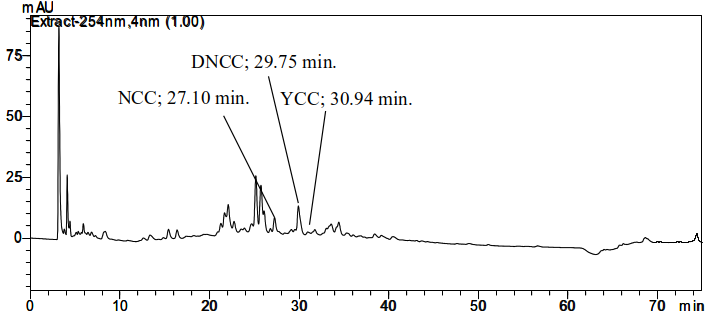
\includegraphics[width=\textwidth]{figures/Kapitel6/keineReaktion/VWA_HPLC_Chromatogramm_keineReaktion.png}
  \caption[HPLC Chromatogramm vor der Reaktion, Quelle: Author]{\gls{hplc} Chromatogramm - die hervorgehobenen Peaks entsprechen den Retentionszeiten und der Art des \gls{Chl-K}, die über ein UV/Vis Spektrum, aufgenommen im online-Modus, bestimmt wurde; gefunden wurden ein \gls{NCC} bei 27.10min. (Abbildung \ref{fig:}), ein DNCC bei 29.75min. (Abbildung \ref{fig:}) und ein YCC bei 30.94min. (Abbildung \ref{fig:})}
  \label{fig:HPLCChromatogramm}
\end{figure}

Über das an die \gls{hplc} gekoppelte Massenspektrometer wurde ebenfalls ein Chromatogramm erzeugt (Abbildung \ref{fig:LCMSChromatogramm}). Die hervorgehobenen Peaks zeigen an, zu welchem Zeitpunkt welcher Katabolit in Bezug auf seine Molekülmasse gefunden wurde. Da das Massenspektrometer erst nach 10min. an die \gls{hplc} gekoppelt wurde, muss man, um die entsprechende Retentionszeit im \gls{hplc} Chromatogramm zu erhalten, zu jedem Zeitpunkt im Chromatogramm des Massenspektrometers (MS Chromatogramm - Abbildung \ref{fig:LCMSChromatogramm}; HPLC Chromatogramm - Abbildung \ref{fig:HPLCChromatogramm}) 10min. dazuzählen. 

\begin{figure}[!htbp]
  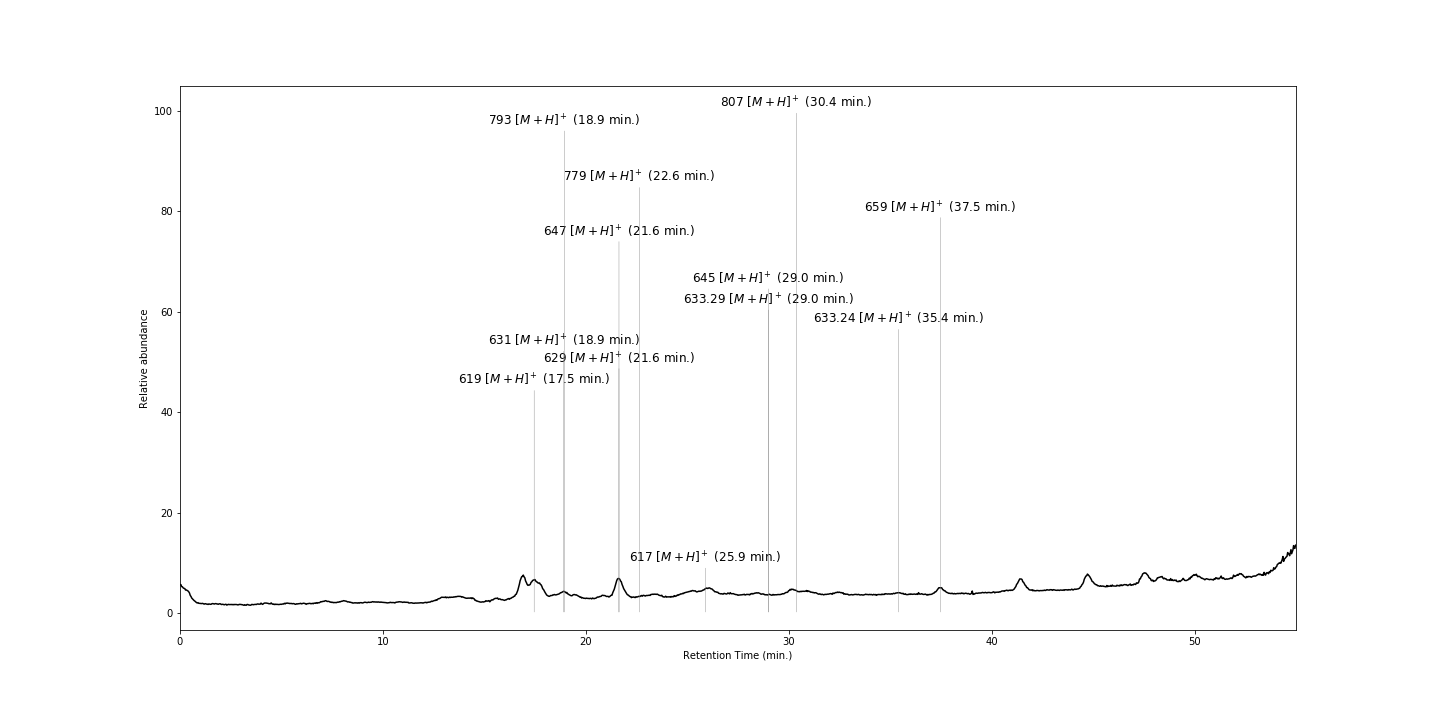
\includegraphics[width=\textwidth]{figures/Kapitel6/keineReaktion/Kuerbis_Analyse_keineReaktion2_Ganzes_Spektrum.png}
  \caption[LC-MS Chromatogramm vor der Reaktion, Quelle: Author]{\gls{lcms} Chromatogramm}
  \label{fig:LCMSChromatogramm}
\end{figure}

Es wurden somit mit dem Massenspektrometer die in Tabelle \ref{tab:LCMSKataboliten} aufgelisteten Phyllobiline identifiziert. In dieser Tabelle werden neben den Summenformeln auch die exakten Massen, die Art des \gls{Chl-K} (NCC, DNCC, YCC, DYCC), die Retentionszeit in der \gls{hplc} (soweit eindeutig feststellbar) angegeben. 

Eine so große Anzahl an \gls{Chl-K} wie in Tabelle \ref{tab:LCMSKataboliten} vorzufinden wäre sehr unwahrscheinlich. Bei einer Betrachtung der Summenformeln und exakten Molekülmassen fällt jedoch auf, dass sich einige \gls{Chl-K} um genau ein C-Atom und zwei H-Atome unterscheiden (entsprich 14Da). Da alle identifizierten Kataboliten eine freie Carbonsäuregruppe an Position .. besitzen, wird angenommen, dass diese bei der Aufarbeitung der Probe mit \gls{meoh} (Kapitel \ref{sec:HPLCAufarbeitungderProbe}) mit diesem reagieren und einen Methylester ausbilden. In der Spalte Herkunft (abgekürzt mit H.) der Tabelle \ref{tab:LCMSKataboliten} wird demnach festgehalten, von welchem \gls{Chl-K} die jeweilige Verbindung stammt. \\

\begin{table*}\centering
  \ra{1.3}

  \begin{tabular}{cccccc}\toprule
 Bezeichnung & Summenformel & M (in Da) & Typ & RT\textsubscript{HPLC} (in min.) & H. \\
\midrule
\rowcolor{black!20} Bo-DYCC & \ch{C33H37O8N4} & 617.2635 & DYCC & 30.94? & - \\
 Bo-DNCC & \ch{C33H39O8N4} & 619.2793 & DNCC & 26.72 & - \\ 
\rowcolor{black!20} • & \ch{C34H37O8N4} & 629.2639 & • & - & - \\ 
 - & \ch{C34H39O8N4} & 631.2795 & DYCC & 29.91, 30.94 & Bo-DYCC \\ 
\rowcolor{black!20} - & \ch{C34H41O8N4} & 633.2955 & DNCC & - & Bo-DNCC \\ 
 • & \ch{C36H33O7N4} & 633.2339 & • & • & - \\ 
\rowcolor{black!20} Bo-YCC & \ch{C34H37O9N4} & 645.2593 & YCC & - & - \\ 
 Bo-NCC-3 & \ch{C34H39O9N4} & 647.2748 & NCC & 33.04 & - \\ 
\rowcolor{black!20} - & \ch{C35H39O9N4} & 659.2741 & YCC & - & Bo-YCC \\
 Bo-DNCC-2 & \ch{C39H47O13N4} & 779.3181 & DNCC & • & - \\ 
\rowcolor{black!20}Bo-NCC-1 & \ch{C40H49O13N4} & 793.3336 & NCC & 29.91 & - \\ 
 - & \ch{C41H51O13N4} & 807.3491 & NCC & - & Bo-NCC-1 \\ 
\bottomrule
  \end{tabular}
  \caption[Übersicht über die Chl-Kataboliten des Brokkoliblattes, Quelle: Author]{Übersicht über die gefundenen Chl-Kataboliten des Brokkoliblattes und ihren Methylestern, die sich aus der Reaktion der freien Carbonsäure mit \gls{meoh} ergeben}
  \label{tab:LCMSKataboliten}
\end{table*}

Im Rahmen meiner Vorwissenschaftlichen Arbeit erwies es sich als schwierig, die Resultate der \gls{hplc} mit denen des Massenspektrometers im Rahmen eines \gls{lcms} Versuches in Einklang zu bringen. Da die Verwendung von Daten aus der \gls{hplc} zur Analyse der \gls{Chl-K} nicht das primäre Ziel meiner Arbeit war, spielt dies auch keine wesentliche Rolle. Aus Gründen der wissenschaftlichen Vollständigkeit, werden die Daten der \gls{hplc} trotzdem präsentiert. Ebenso wird versucht, die Probleme, die sich aus den Daten ergeben, zu erklären.

Der Typ des \gls{Chl-K} wurde, sofern dies möglich war durch ein UV/Vis Spektrum im Onlinemodus bestimmt und mit der vom Massenspektrometer erhaltenen Summenformel und den sich daraus ergebenden strukturellen Möglichkeiten überprüft. War die Zuordnung anhand UV/Vis Spektren aufgrund von Unklarheiten nicht möglich, wurde zur Strukturbestimmung auf die Daten des Massenspektrometers zurückgegriffen.\\

Bei einer Retentionszeit von 27.10min. konnte über UV/Vis ein \gls{NCC} (Abbildung \ref{fig:NCC2725}) identifiziert werden, da er bei einer Wellenlänge von 315nm eine charakteristische Bande aufweist. Der von den Retentionszeiten dazugehörige \gls{Chl-K} im Massenspektrum wäre der Bo-DNCC (mit einer Retentionszeit von 17.5min im Massenspektrometer - Abbildung \ref{fig:LCMSChromatogramm}). Bei diesem handelt es sich jedoch um einen \gls{DNCC}. Es wurde versucht, das unlogische Ergebnis durch Überlagerungen mehrer \gls{Chl-K} zu erklären, was aber nicht möglich war (Abbildung \ref{fig:}). Es bleibt somit das zustandekommen dieses UV/Vis Spektrums ungeklärt. 

Bei einer Retentionszeit von 29.75min. konnte ein UV/Vis Spektrum eines \gls{DNCC}s (Abbildung \ref{fig:DNCC2991} aufgenommen werden. Nach den Retentionszeiten im Massenspektrometer (Abbildung \ref{fig:LCMSChromatogramm}) kann diesem UV/Vis Spektrum der \gls{Chl-K} Bo-NCC-1 zugeordnet werden. Auch der Methylester des Bo-YDNCC ist zu dieser Retentionszeit im Massenspektrometer vorzufinden und trägt damit vermutlich zur Entstehung des Signals bei, was die Verzerrungen bewirken könnte.

Bei einer Retentionszeit von 30.94min. ist das UV/Vis Spektrum charakteristisch für einen \gls{YCC} (Abbildung \ref{fig:DNCC2991}). Im Massenspektrometer wurde zu dieser Retentionszeit der Methylester des Bo-YDNCC gefunden (bei einer Retentionszeit von 18.9min). Auch hier lässt sich keine Verbindung finden, bei der die Retentionszeiten von \gls{hplc} und Massenspektrometer exakt zusammenpassen. Es könnte auch hier wieder zu einer Überlagerung kommen (vielleicht mit dem Bo-YDNCC). Diese Überlagerungen könnten durch Isomere der einzelnen \gls{Chl-K} bedingt sein. \\

\begin{figure}[!htbp]
  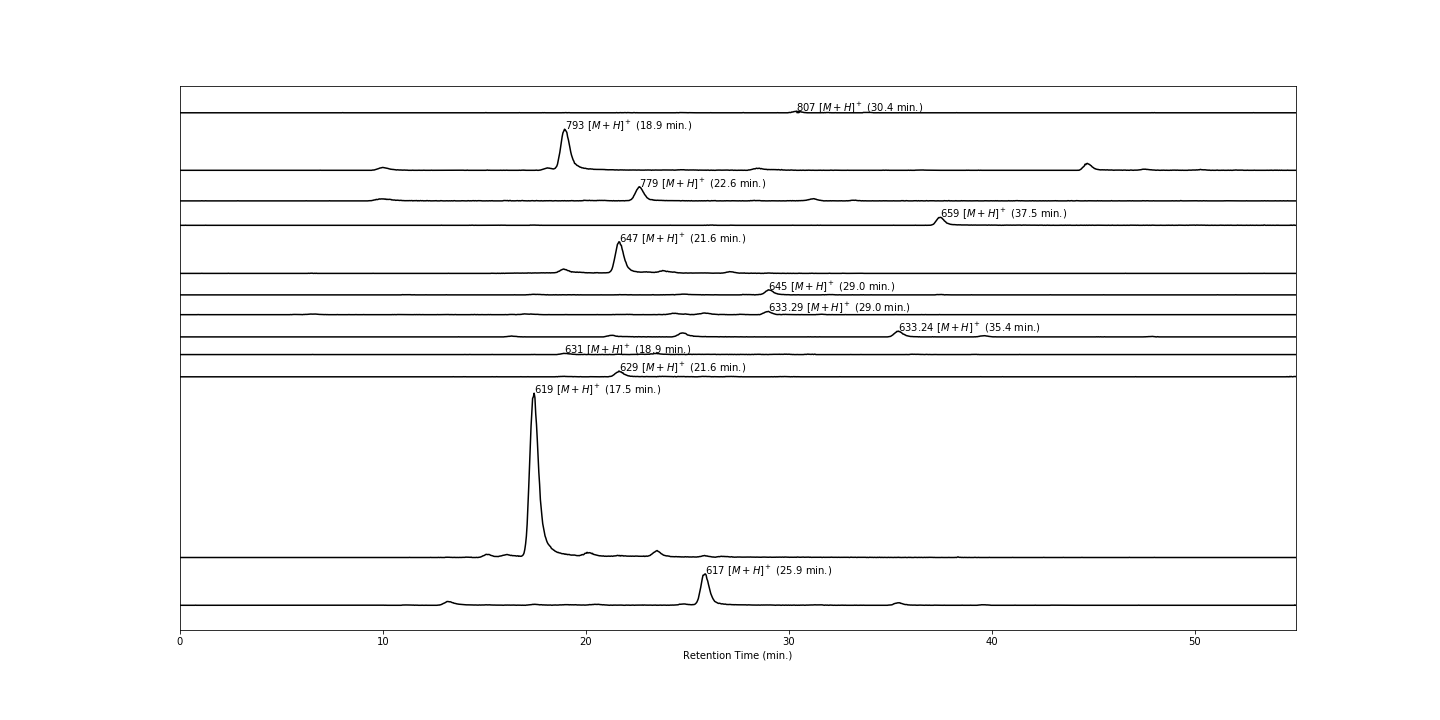
\includegraphics[width=\textwidth]{figures/Kapitel6/keineReaktion/Kuerbis_Analyse_keineReaktion2_LC-ESI-MS.png}
  \caption[LC-MS Chromatogramm Aufspaltung, Quelle: Author]{\gls{lcms} Chromatogramm}
  \label{fig:LCMSChromatogrammAufspaltung}
\end{figure} 

Um das Zustandekommen der nicht identifizierbaren UV/Vis Spektren zu erklären wurden Diagramme wie in Abbildung \ref{fig:LCMSChromatogrammAufspaltung} erstellt. Es handelt sich dabei um ein Chromatogramm jedes einzelnen im Massenspektrometer während eines \gls{lcms} Laufes identifizierten \gls{Chl-K}. Die Intensitäten wurden auf den höchsten im Zeitraum vorkommenden Peak skaliert. Bei den gekennzeichneten Peaks handelt es sich um jene, bei denen die jeweilige Verbindung die höchste Intensität im Chromatogramm zeigte. Mithilfe dieser Abbildung sollten etwaige Überlagerungen herausgefunden werden. 

\begin{figure}[!htbp]
  \begin{subfigure}[b]{0.5\textwidth}
    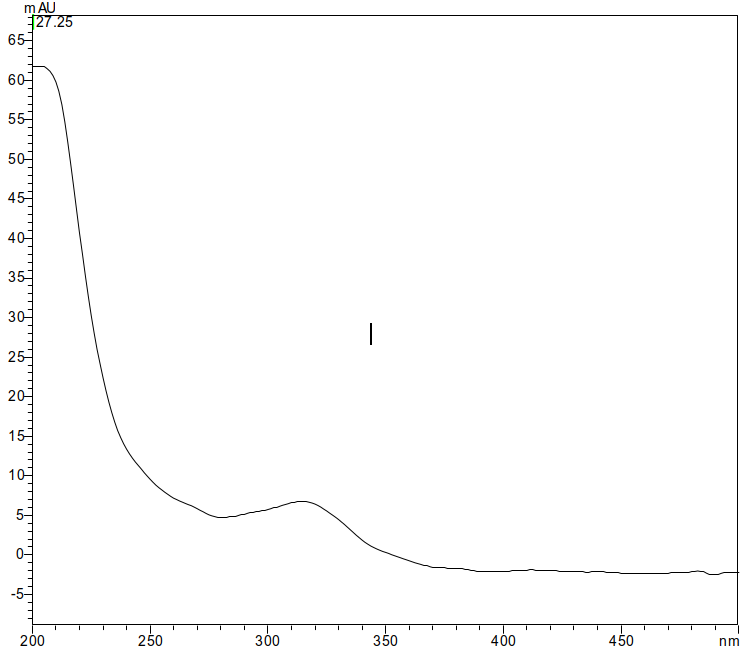
\includegraphics[width=\textwidth]{figures/Kapitel6/keineReaktion/NCC2725.png}
    \caption{}
    \label{fig:NCC2725}
  \end{subfigure}
  \hfill
  \begin{subfigure}[b]{0.5\textwidth}
    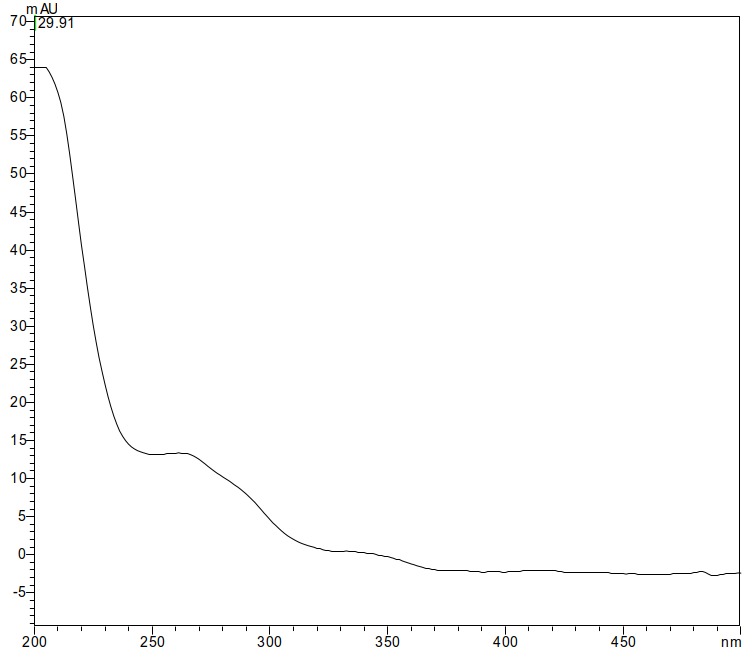
\includegraphics[width=\textwidth]{figures/Kapitel6/keineReaktion/DNCC2991.png}
    \caption{}
    \label{fig:DNCC2991}
  \end{subfigure}
  
  \begin{subfigure}[b]{0.5\textwidth}
    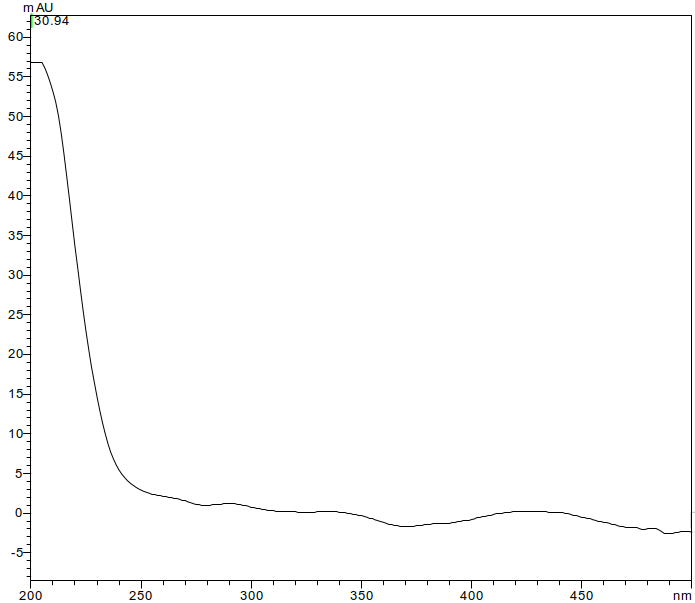
\includegraphics[width=\textwidth]{figures/Kapitel6/keineReaktion/YCC3094.png}
    \caption{}
    \label{fig:DNCC2991}
  \end{subfigure}
  \caption[UV/Vis online Spektren mit der Charakteristik eines NCC bei 27.10min., eines DNCC bei 29.75min. sowie eines YCC bei 30.94min., Quelle: Author]{UV/Vis online Spektren: (a) charakteristisch für einen \gls{NCC} - RT = 27.25min., (b) charakteristisch für einen \gls{DNCC} - RT = 29.91min., (c) charakteristisch für einen \gls{YCC} - RT = 30.94min.}
\end{figure}
